\documentclass[letterpaper,10pt,onecolumn]{IEEEtran} %!PN

\usepackage{graphicx}    
\usepackage{epstopdf}  

\usepackage[justification=centering]{caption}

\usepackage{amssymb}                                         
\usepackage{amsmath}                                         
\usepackage{amsthm}                                          

\usepackage{alltt}                                           
\usepackage{float}
\usepackage{color}

\usepackage{hyperref}
\usepackage{url}

\usepackage{balance}
\usepackage[TABBOTCAP, tight]{subfigure}
\usepackage{enumitem}

\newcommand{\ignore}[2]{\hspace{0in}#2} %Used for inline comments
\newcommand{\tab}{\hspace*{2em}} %For tabbing

\usepackage{pstricks, pst-node}

\usepackage{geometry}
%\usepackage{graphicx}
\geometry{textheight=10in, textwidth=7.5in}

\usepackage{listings}

\definecolor{mygreen}{rgb}{0,0.6,0}
\definecolor{mygray}{rgb}{0.5,0.5,0.5}
\definecolor{mymauve}{rgb}{0.58,0,0.82}

\lstset{ %
  basicstyle=\ttfamily,            % the size of the fonts that are used for the code
  breakatwhitespace=false,         % sets if automatic breaks should only happen at whitespace
  breaklines=true,                 % sets automatic line breaking
  captionpos=b,                    % sets the caption-position to bottom
  commentstyle=\color{mygreen},    % comment style
  escapeinside={\%*}{*)},          % if you want to add LaTeX within your code
  extendedchars=true,              % lets you use non-ASCII characters; for 8-bits encodings only, does not work with UTF-8
  keepspaces=true,                 % keeps spaces in text, useful for keeping indentation of code (possibly needs columns=flexible)
  keywordstyle=\color{blue},       % keyword style
  numbers=left,                    % where to put the line-numbers; possible values are (none, left, right)
  numbersep=10pt,                  % how far the line-numbers are from the code
  numberstyle=\tiny\color{mygray}, % the style that is used for the line-numbers
  rulecolor=\color{black},         % if not set, the frame-color may be changed on line-breaks within not-black text (e.g. comments (green here))
  showspaces=false,                % show spaces everywhere adding particular underscores; it overrides 'showstringspaces'
  showstringspaces=false,          % underline spaces within strings only
  showtabs=false,                  % show tabs within strings adding particular underscores
  stepnumber=1,                    % the step between two line-numbers. If it's 1, each line will be numbered
  stringstyle=\color{mymauve},     % string literal style
  tabsize=8,                       % sets default tabsize to 8 spaces
  %title=\lstname                  % show the filename of files included with \lstinputlisting; also try caption instead of title
}

\usepackage{hyperref}

\def\BibTeX{{\rm B\kern-.05em{\sc i\kern-.025em b}\kern-.08em
    T\kern-.1667em\lower.7ex\hbox{E}\kern-.125emX}}

\begin{document}

%\title{Using the Style File IEEEtran.sty} 
\title{Tools for Supporting Community Growth in Open Source } %!PN

\author{Bruntmyer J. Author, OSU, Goossens M. Author, OSU, Nguyen H. Author, OSU}

\markboth{IEEE Transactions On Automatic Control, Vol. XX, No. Y, Month
1999}
%{Murray and Balemi: Using the style file IEEEtran.sty} %!PN
{Murray and Balemi: Using the Document Class IEEEtran.cls} %!PN


\maketitle
%\thispagestyle{plain}\pagestyle{plain}

\begin{abstract}
For 13 weeks our group has been working on a project that is creating tools that gives users the ability to look for open source community leaders that are hosting events about projects that they are leading. These tools will allow users to have the opportunity to find these events in order to become a contributor to an open source project. This is done in a form of a website that will have features for finding certain events dealing with open source projects so that it can be easily accessible by people with a passion for wanting to contribute to projects. Throughout this document, we look at what this team has accomplished for each of the requirements we have laid out, discussing problems that have halted our progression through the project, and what we have left to do before completion of the project. We are currently at a strong alpha level stage for this project as we continue to develop for our beta and version 1.0 stages. Also included are important images of the user interface we have decided to use, along with pieces of code that we have completed and worked with thus far. By the end of this document, you will get a complete picture of how we reached our alpha level prototype and what we have left to finish before we have a version 1.0 ready to be used.
\end{abstract}

\newpage

\section{PROJECT PURPOSES AND GOALS}
After working on the project for about five weeks now, the perspective on what the community development tool wants to accomplish becomes much more abundantly clear. After taking much more time to read and understand much of the code that was previously written for the prototype, we can see more clearly on how exactly the data is organized and connected using Django and its tools. First and foremost, the purpose of the community development tool remains the same. The purpose is to gather information from meetup.com and parse that information into a list of upcoming events related to Apache and open source projects so that developers in the open source community have an easy to access environment where they can hope to participate in those events to further help the ongoing development for a certain project. The original goals of the project remain the same in hopes to accomplish this complete tool that implores self-sufficient developers to read about updated events and engage with the community leaders that are hosting the events and projects.

\section{CURRENT PROGRESSION THROUGH REQUIREMENTS}

\subsection{Fix the “People” page where the list of community leaders are shown}
\begin{enumerate}[label*=\arabic*.]
\item Current Progress: The “People” page currently takes all of the people in the database and lists them onto the page. Normally, if the prototype is hosted on a local machine and the database is relatively small, then the page loads fine in a minimal amount of time. The issue is nested in the actual hosted site by Apache where hundreds of thousands people are imported into the database daily and dramatically slowing down the loading time of the page. With our current progression of the project, we have not made significant progress into improving the loading time of the page. We use our own local host to import a small amount of members at a time and that requirement is set to be worked on shortly for Beta implementation. The guideline for working towards accomplishing this requirement is to limit the amount of people loaded at a time onto the page. For Beta, we have rearranged where the table is generated for the people page in the function within views.py. This change specifically was introduced because a bug was found where when the table is generated, then if the amount of people were too many, then the table would crash and not build. With the rearrangement, now the table does not break through a large build and now tends to load faster.

\item Things to Complete: Currently, the implementation of the fix for the People page is local. We have not yet successfully pushed it onto the hosted paged by Apache yet as it is still in progress to be reviewed. This means that any kind of test for speed and efficiency is scaled down and need still need more kinds of testing. Once the implementation is approved, then we can test this feature on a larger scale and look for more tendencies on where execution fails for further improvement.
\end{enumerate}

\begin{figure}[htp]
  \begin{center}
  
  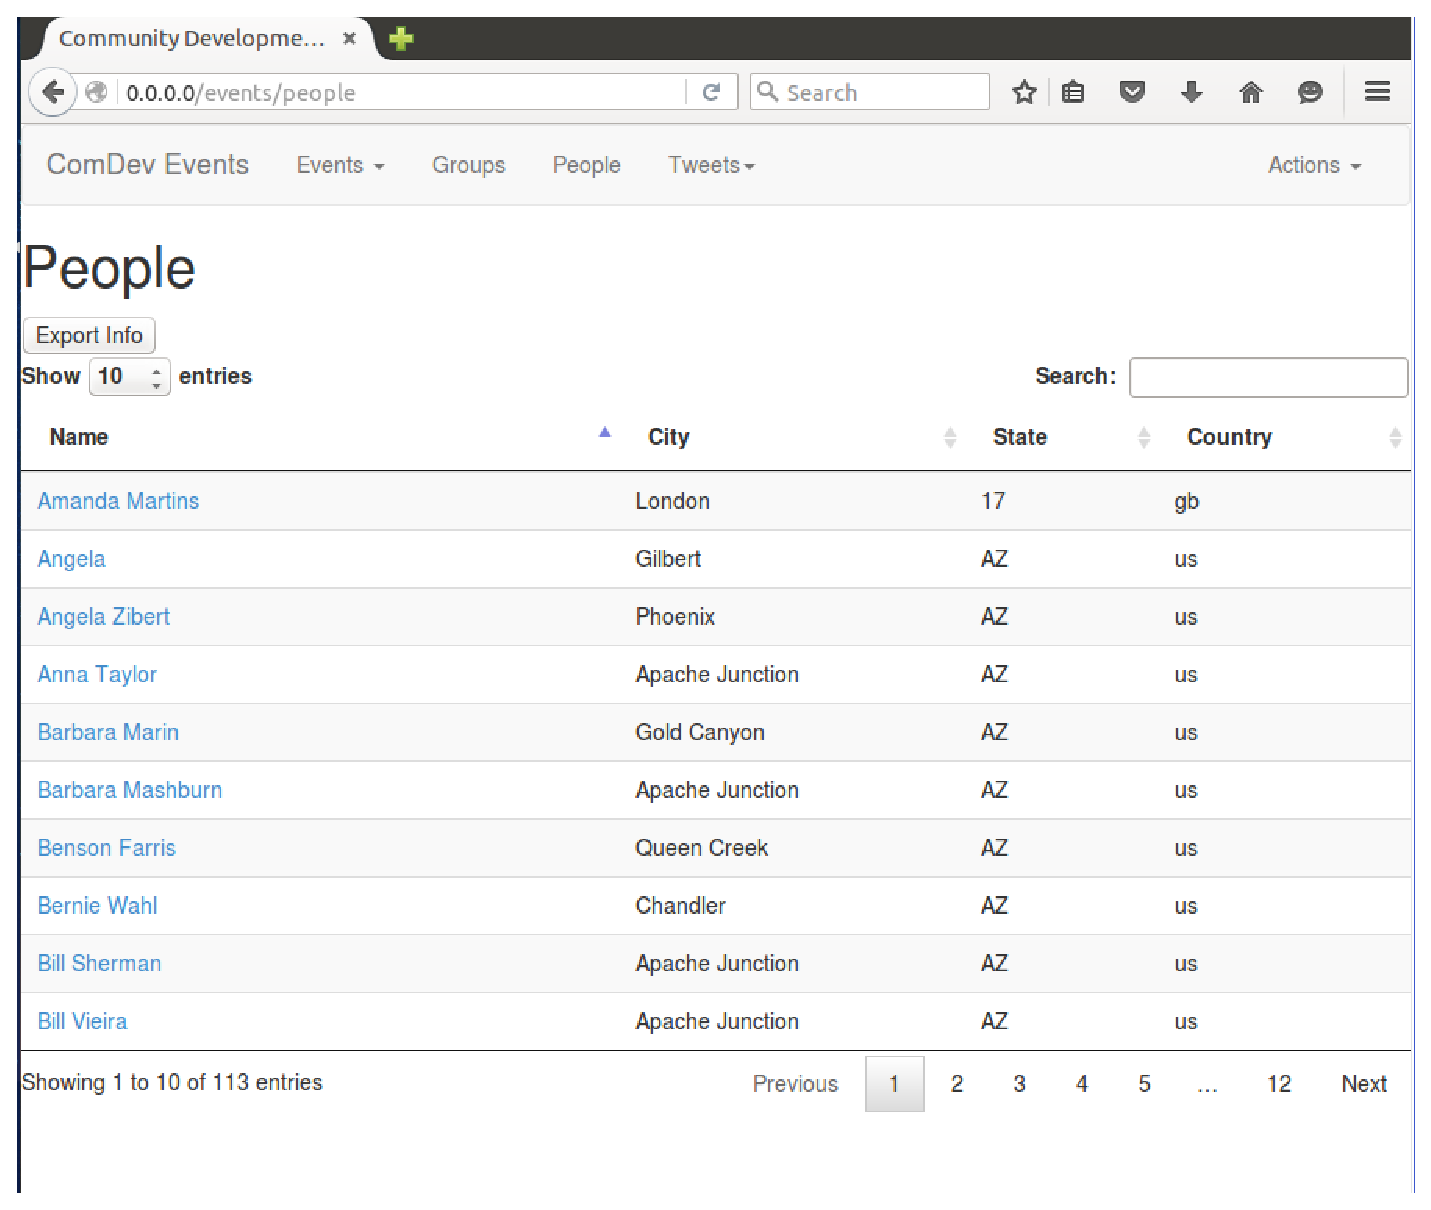
\includegraphics[width=2in]{peoplePage}
  \centering
  \caption{The people page}

  \end{center}
\end{figure}

\subsection{Tweet at a person listed in the database}
\begin{enumerate}[label*=\arabic*.]
\item Current Progress: Currently, a person is generated their own profile page based off of their Meetups ID and information from meetups about the person’s profile is also parsed in the community development tool. The purpose of this requirement is for the self-sufficient programmers interested in a certain event or project to be given the tools to communicate with leaders and members in those groups to begin their own development on the projects. A button to tweet at the person is currently implemented for the profile generated page where the user should be able to click on the tweet at the person using their Twitter handle.

\item Things to Complete: There is no current variable that retains the generated person’s twitter profile. That information is still held within meetups but that information is not yet parsed correctly. Our goal is to generate that information correctly so that the user can be directed to the correct Twitter page and if that person does not provide their Twitter page, then the user would be directed to the group of the person’s Twitter handle. If that group does not have a Twitter, then the option to tweet should not be provided.
\end{enumerate}

\begin{figure}[htp]
  \begin{center}
  
  
\includegraphics[width=2in]{tweet_person1}
  \centering
  \caption{The button that is displayed when a user has a twitter handle that is publicly available on Meetups that allows a user to tweet at the person.}

  \end{center}
\end{figure}

\begin{figure}[htp]
  \begin{center}
  
  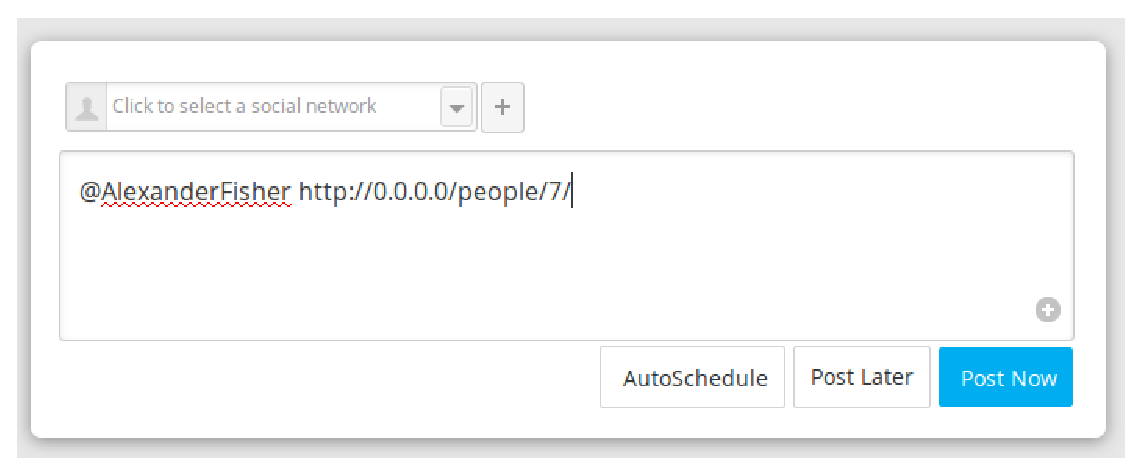
\includegraphics[width=2in]{tweet_person2}
  \centering
  \caption{The HootSuite service is used to send the tweet at the person as we supply the twitter handle and it is up to the user to use their Twitter account to tweet.}

  \end{center}
\end{figure}

\subsection{Add user accounts to application and track when a user has tweeted an event}
\begin{enumerate}[label*=\arabic*.]
\item Current Progress: The purpose to adding user accounts to the application is to be able to have an input and contribute to keep track of all of the users and tweets that they have posted about Apache and open source material. Although this is currently the only purpose of the user account as time allows through the requirements, the use of having access to a login and account is still important and can be branched out to many other purposes following continued development on the application. Another possible use through a stretch goal for the account is to add their own nearby location through location services so that when the user navigates to the Geo-Location page, then the website will automatically locate an event based on their location. For the purpose of tracking when a user has tween about an event. It is useful because it gives more information available for people to track activity on topics that people care about and invest their time to develop. Our current development at this stage contains the main account creation page where users can click on and go to on the website. Currently once that information is submitted, the website has yet to complete the application and leads to a “in current development page.”

\item Things to Complete: The application still has yet to complete the database side of the addition of the user accounts. The user has access to the account creation page, but anything that they enter will not be stored into the database yet because that it is not yet implemented. Also, other main attributes of what the account should contain such as “TwitterID”, “Account locations” and other various variables are still have yet to be decided and implemented via the application.
\end{enumerate}

\begin{figure}[htp]
  \begin{center}
  
  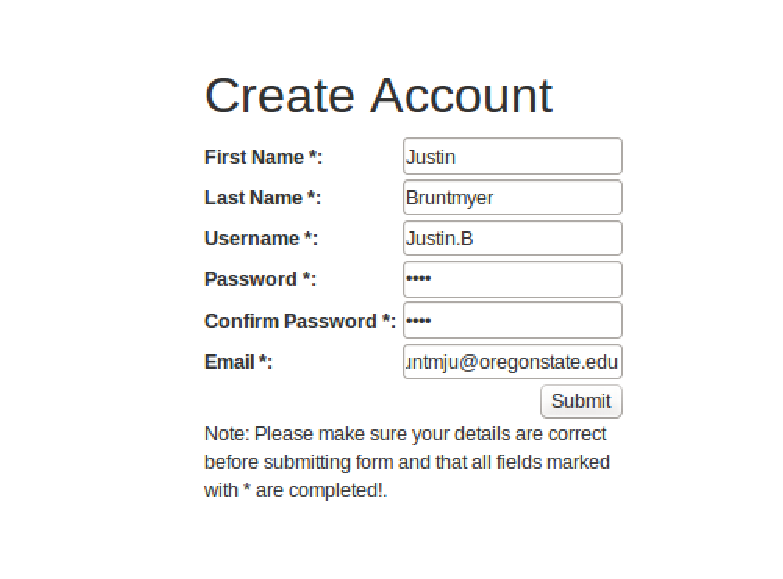
\includegraphics[width=2in]{createAccountForm}
  \centering
  \caption{Example usage of the create account form. }

  \end{center}
\end{figure}

\begin{figure}[htp]
  \begin{center}
  
  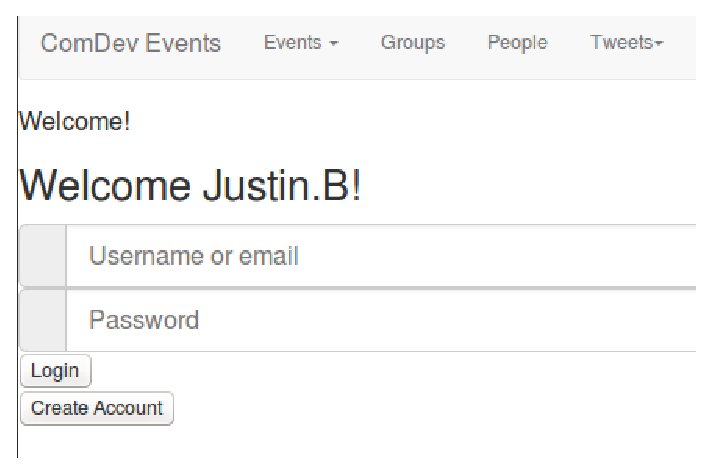
\includegraphics[width=2in]{loginSuccess}
  \centering
  \caption{Showing created user actually signing into the website. }

  \end{center}
\end{figure}

\subsection{List tweets about events and/or people via the application}
\begin{enumerate}[label*=\arabic*.]
\item Current Progress: When an event is viewed by a user, a button is available so that the user can tweet about the event if they choose so. Current progression on the application has the button available, but currently does not link to the correct page for Twitter to access the user’s account to automatically generate the Tweet for the user. The intention of this purpose is to gain more publicity that is readily available for the user through auto-generated tweets and hashtags for more people to see and to introduce more traffic.

\item Things to Complete: This button would be utilized by the web tool Hootsuite, an application that would have access to the user’s Twitter account if they have it saved on their web browser. Hootsuite would generate an automated tweet such as “This great open source event is coming up! Come read more about it here! via (our web application).”
\end{enumerate}

\subsection{List tweets about events and/or people not via the application}
\begin{enumerate}[label*=\arabic*.]
\item Current Progress: Currently, the website parses events that are listed through meetup.com. We want to extend this feature as well through Twitter so that it reads any tweets related to a relevant event that is posted. If a certain hashtag is used, then the application picks up that tweet, parses the information through the tweet itself and the user that tweeted it. This parser is not yet built and still is under current development. There is currently a button on the application under the navigation tool where the user and click on to view all tweets, but currently no data has been parsed yet for the tool.

\item Things to Complete: We still need to develop the parser for the tweet and extend that for the webpage tool. The tool should look like an organized list that has all tweets listed in chronological order starting from the most recent. Eventually, there should be a category of tweets based on hashtags relevant for what topic the user wants to see.
\end{enumerate}

\begin{figure}[htp]
  \begin{center}
  
  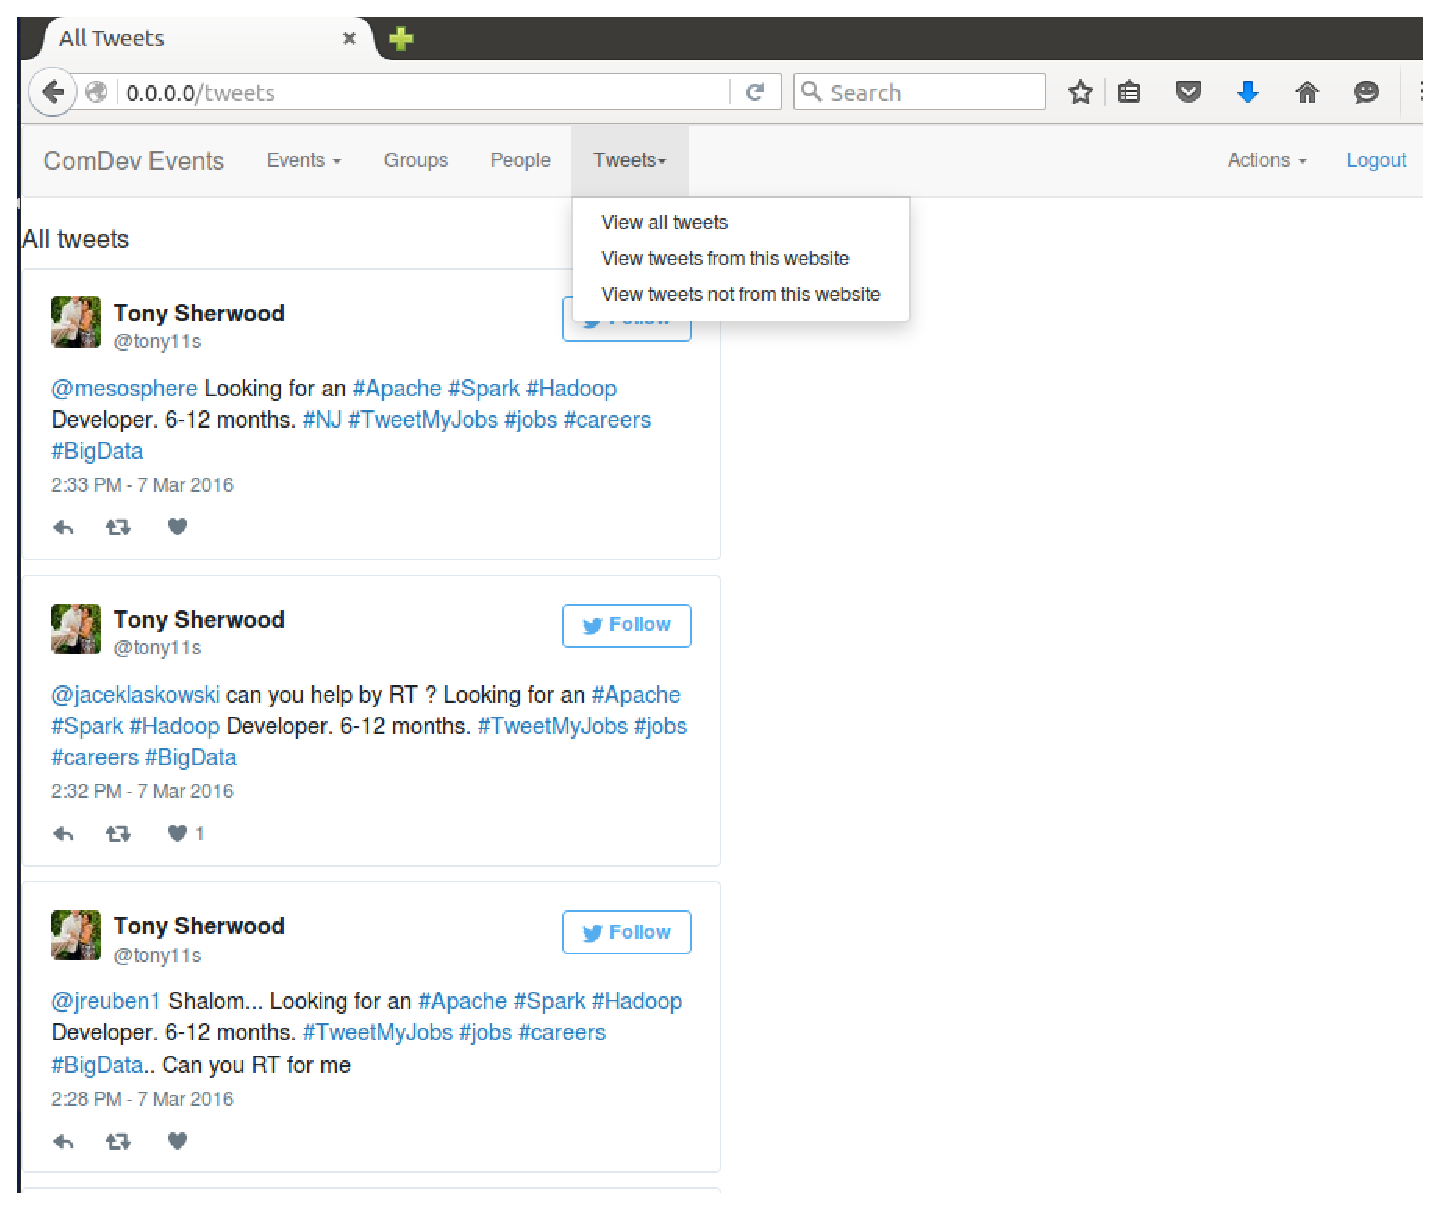
\includegraphics[width=2in]{listingTweets}
  \centering
  \caption{Showing our application listing the tweets that are located on twitter. }

  \end{center}
\end{figure}

\subsection{Export a list of people and email addresses}
\begin{enumerate}[label*=\arabic*.]
\item Current Progress: The only possible input actions that users are allowed is the ability to import events and group members for the current application. A very useful tool that could be included is the ability to export a list into a csv for all people and their email addresses that are in a community group so that the user has that tool to contact any person from there. An issue that has come across through looking at the nature of meetup parsing and the current application is that we are unable to parse emails from users that are in groups because that information is simply not available. This halts the process in being able to export that part of the list and we may have to re-purpose this requirement. Under the “people” page, there is a button available for the user to click on intended for this requirement but has not yet been fully implemented.

\item Things to Complete: In terms of completion of this requirement, we still need to fully implement the export function of this button. Functionally only leads the user to a blank page and it does not yet generate the needed information from the database. This requirement should not be an issue to complete, the task will be more trivial compared to the other requirements.
\end{enumerate}

\begin{figure}[htp]
  \begin{center}
  
  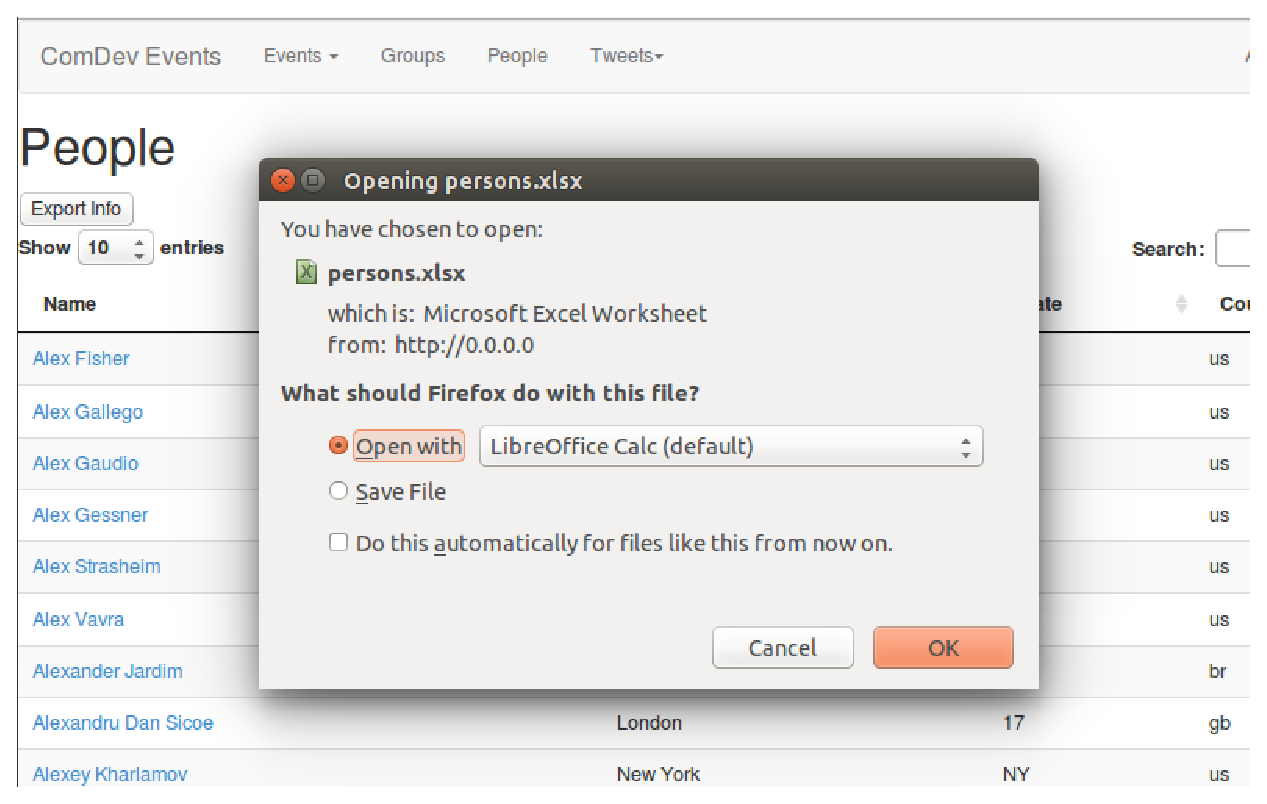
\includegraphics[width=2in]{exporting1}
  \centering
  \caption{Showing export button executing. }

  \end{center}
\end{figure}

\begin{figure}[htp]
  \begin{center}
  
  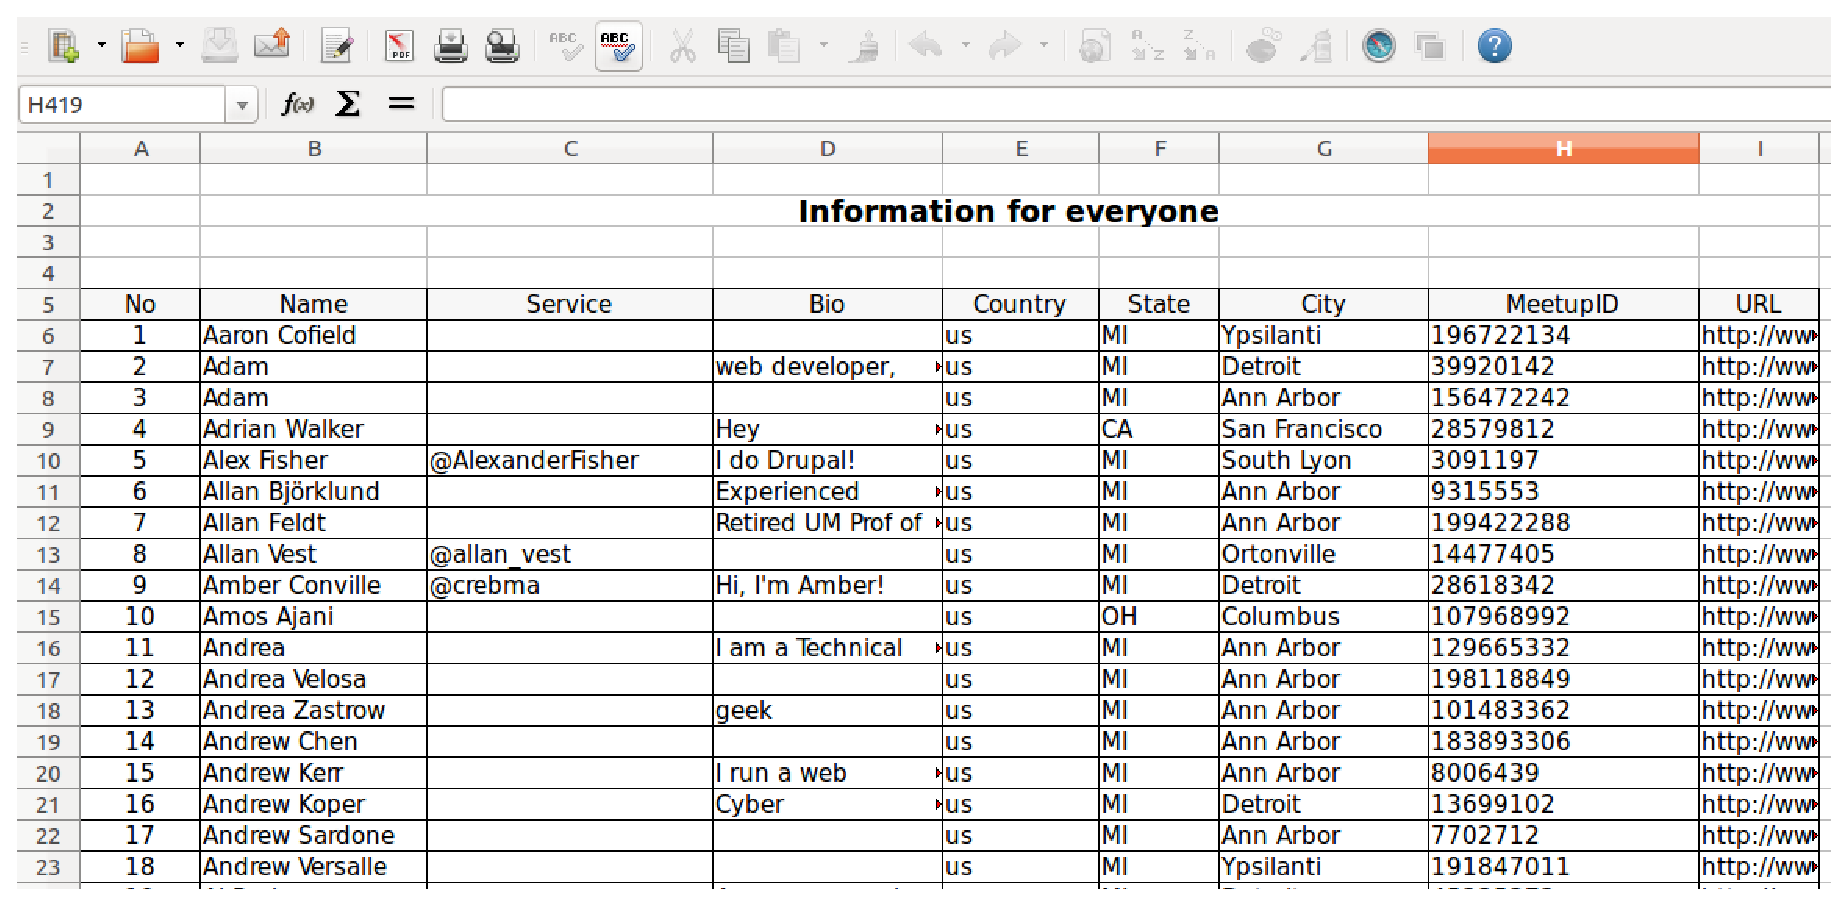
\includegraphics[width=2in]{exporting2}
  \centering
  \caption{Showing the list of exported information about people that were imported. }

  \end{center}
\end{figure}

\subsection{Improve hashtag searching of application to improve finding more relevant events}
\begin{enumerate}[label*=\arabic*.]
\item Current Progress: The web application currently successfully parses information from events that are in any way related to Apache and open source development. The issue at hand is that around 50 percent of the events parsed are also completely unrelated meetup events that do not have the same development intention of the application such as mountain bike racing and hiking events. These types of events are also parsed through the application which thus calls for the improvement of the searching algorithm for finding more relevant events. Currently the webpage has the tool to mark events not applicable which would remove the event completely from the list of events. This is a good short term solution for the current day, but it is not an automated process and marking relevant events not applicable is also very possible. In order to improve the available sorting of more relevant events, we need to develop a more viable option still.

\item Things to Complete: The intended solution looks at how the information is gathered. Currently the searching of the application looks for keywords. In this case the keyword is the hashtag of Apache. Any event that has the word Apache in it will thus then show up the in the event list. Oddly enough, there are some events even still that show up on the list which do not even contain the keyword Apache. Our solution is to create filter keywords that remove events that have a keyword that is not related to the intention of the application. We will also create a more broad range of keywords to search for to view events as well. This will hopefully improve the amount of events that are more relevant to open source development.
\end{enumerate}

\subsection{Improve the visuals of the tool's look as a whole}
\begin{enumerate}[label*=\arabic*.]
\item Current Progress: The application itself is fairly organized at the moment. The navigation bar implementation really helps the user keep track navigating between each page. When viewing the list of events, the events are listed in chronological order starting with the most recent. There is a search bar available for the user to type in for a certain event that they wish to view. There are other sorting mechanisms to view those events in another sorting order. However, there are some elements missing that could still be improved to help users navigating on the webpage. There are a few improvements that still should still be implemented to overall help the feel of the website.

\item Things to Complete: When viewing a single event, all the relevant information is parsed and organized well for the user to view, but it is in a plain text format. Functionally, this is great, but the page itself can still be improved to make the page look more appealing and easier to view. This can be applied to viewing a specific person as well. There a few pages missing still that need to be created such as a page that contains information about a specific group. This page would be especially useful for users wishing to learn more about a specific group or community to start to get involved in.
\end{enumerate}

\subsection{Implement system of improved sorting of finding events by nearby location within radius of the user}
\begin{enumerate}[label*=\arabic*.]
\item Current Progress: The current tool has the function to create a list of all events parsed through the application and the ability to search for a specific event by sorting or an individual search. An additional option is added for the user to be able to locate an event based on the location that they input within a certain mile radius of that location. The current implementation of this requirement has the searching bar created, but does not yet have the implementation of the actual searching algorithm ready.

\item Things to Complete: Since Apache is open source, some implementation of a searching tool has already been implemented for another project. With that implementation available for reference, the implementation for the application should be in a similar fashion; however, there has been a large issue for this development because the code written is not in the same version of Django as our current application. In addition, trying to understand the implementation for the location services is very difficult to fully comprehend to implement that onto the application. After spending three weeks on trying to implement that portion of the feature, we have not yet been successful and are starting to try to approach this feature in a different method. Django has geo-location services that is actually already in its system, so we are currently looking at that as an alternative option.
\end{enumerate}

\begin{figure}[htp]
  \begin{center}
  
  \includegraphics[width=2in]{mapSearching}
  \centering
  \caption{Showing the map of where you can search a location to see nearby events, also listing events locations. }

  \end{center}
\end{figure}

\subsection{Add feature to generate a profile for people and have it display a way to contact the person if a method is available}
\begin{enumerate}[label*=\arabic*.]
\item Current Progress: The main goal of the tool is to promote community development in the open source scene. A very important feature is then to have the best information available for users who would like to start development to be easily viewable. With a generated profile for community developers to have their contact information, this eases the process for users in which they can start engaging in the community. Our current implementation with these profiles are the “people” pages in which information about the person is available. Contact information about that specific person is not entirely parsed through and may have to be manually implemented. This part of the feature has been highly discussed within the group as many concerns have come up such as how a user would identify themselves as a community developer or community leader. Permissions that a user would have to add their own events have been discussed but ultimately dismissed because of certain attributes that are undesirable such as

\item Things to Complete: Before fully implementing this system, the issue at the hand is to fully distinguish what part of this development tool will it belong in and who the intended population is. It is important to have community leaders to have their contacting information for the public to see, but it is also dangerous to allow just any individual to post something on an open webpage.
\end{enumerate}

\begin{figure}[htp]
  \begin{center}
  
  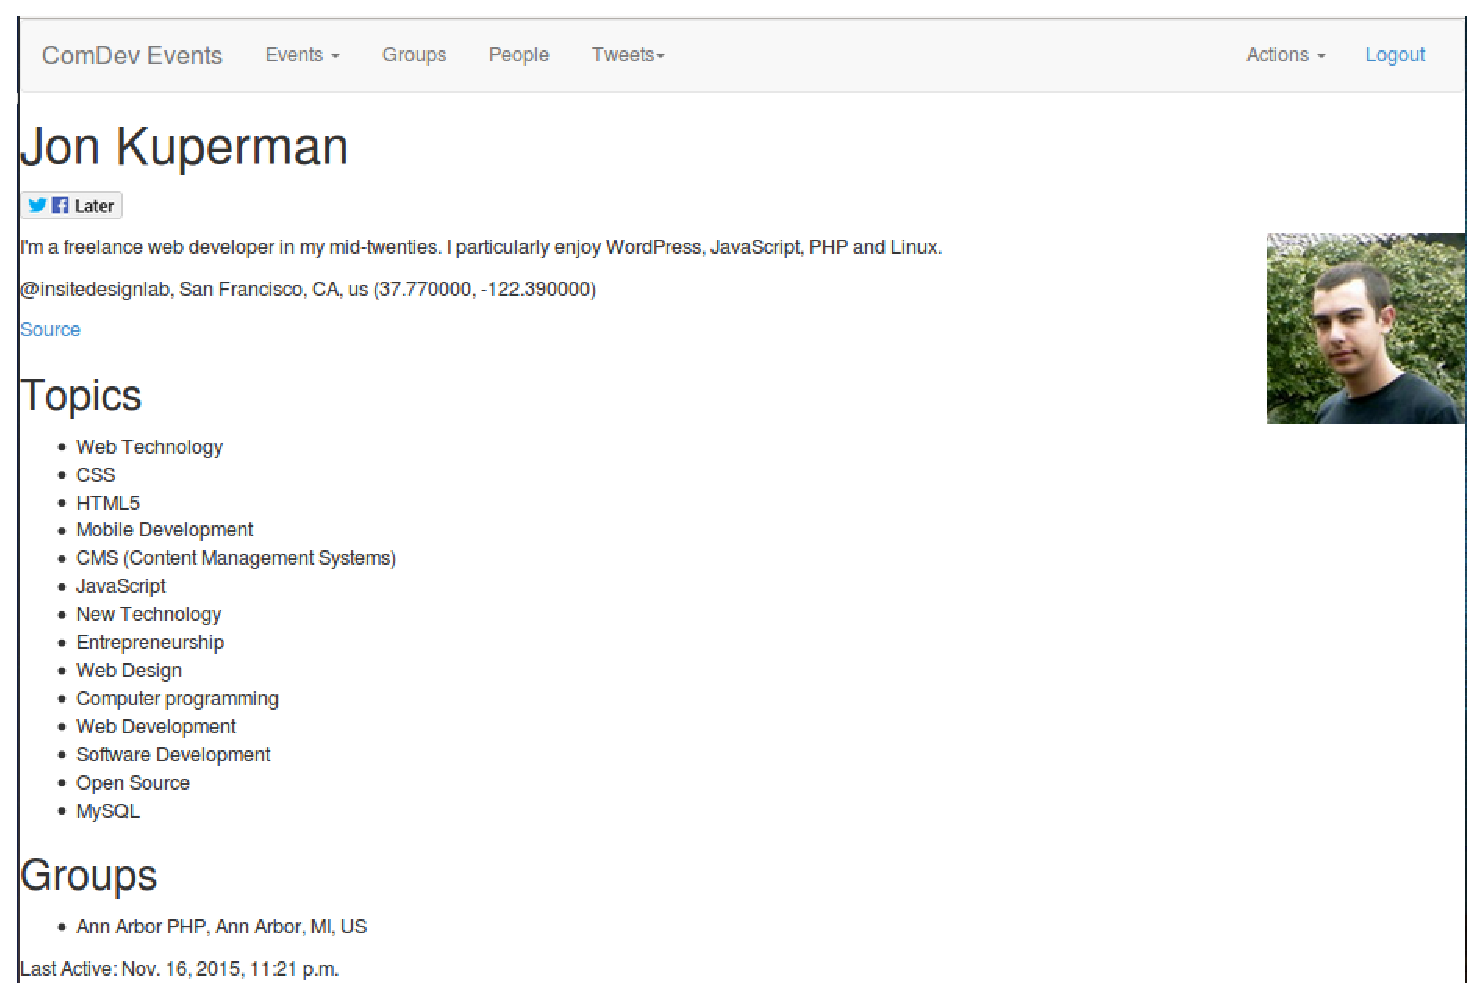
\includegraphics[width=2in]{peopleProfile}
  \centering
  \caption{Showing profile generated for person along with a twitter handle for a method of contacting. }

  \end{center}
\end{figure}

\section{PROBLEMS ENCOUNTERED}

Throughout this term we have encountered many problems that have impeded our progress for this project. This was to be expected as with all projects events occur that can halt progress and bring forth challenges that, as a group, we needed to overcome. The problems that we have faced are listed below along with the methods we used to get through the situation.

\subsection{Problem 1}
Deciding which platform we were going to be developing on using Docker. This was a major issue as we originally planed to work with the Windows operating system however we could not get the application to run locally on a Windows platform. We continually ran into errors with creating a local database along with having the right Docker tools to support the application. We had available resources such as a readme file that gave insight on the problem but whatever we tried did not seem to work. We eventually shifted gears and decided to try Docker and the application on Linux, specifically Ubuntu 14.04. Thanks to the Linux knowledge of Megan Goossens and plenty of online documentation we were able to get Docker installed successfully along with running the application on a local host. From this point we decided to continue developing in the Linux environment.

\subsection{Problem 2}
At the end of the Fall 2015 term we set up a weekly meeting with our client throughout Winter 2016 to discuss implementation details for the week and planned to utilize this time to make sure everyone is on the same page. Due to some miss-communication we were unable to meet with our client for the first two weeks. This halted our progress with because we had a lot of issues with getting Docker to work with Windows and we were counting on a meeting with our client to resolves those issues as soon as possible. We eventually got in contact with our client and figured out what was happening as the first week our client was on an unexpected trip to the UK and in the second week our client did not realize that these meetings occurred every week throughout the term. These things happen and once we all had a chance to get on the same page every weekly meeting is going smoothly.

\subsection{Problem 3}
During week three of Winter 2016 we ran into the issue of meetings being canceled due to illness and injury. One of our team members experience an injury that caused a full group meeting with a TA to occur which halted our progress in having to get everyone caught up on the same page. This same week another group member became sick and could not make it to two meetings for the week which meant that two people could not make it so two meetings were canceled out of the weekly three meetings we have as a group. This was not too untactful as we were able to work individually at home but it was still a noticeable disruption from the normal work we produce in a week. It did not seem like it was going to effect the group at first however when we began to get back on track it took some adjustments to makes sure everyone was on the same page and try to make up for the week we missed.

\subsection{Problem 4}
During the first week of the term we began developing based on the requirements we had listed in our requirements document. The problem we ran into here was that we had issues understanding what are requirements were trying to say thus we went through the document and changed the language used for the requirements. This did not change the requirement but it made it easier to understand if someone is reading through it. This took a days worth of progress which was frustrating due to the fact that we believed to have this done last term. We currently are happy with the updated requirements document as it has been approved by our client, professor, and TA. This halted our progress by being an unnecessary step in the implementation process as it should have been completed last term.

\section{TIMELINE UPDATE}
When we began the development side of the project we realized that it was best to strive for achieving alpha level functionality with all of our features that we would like to have. This required us to take a different approach then what our timeline originally suggested. With a lot o the dates listed in our timeline included completion of features we did not follow this model as instead we developed simple functionality of user interactions of the features but they did not actually get completed.
Now we are going to focus our attention on getting beta level functionality for each of our features. This means that we will move on from the expected completion date even if that feature is experiencing bugs that we have yet to solve as we will need to get the features to a beta level functionality. Below shows our future timeline for getting these items completed for beta.

\section{USER STUDIES}
Throughout the processes of setting all the features up for the alpha presentation we have been able to get a couple of users to test out our website and give feedback of their experience with out tool. A list of questions was created for these user tests and the feedback has been helpful thus far. We asked the participant to look for projects that they would like to be a part of and try to learn about members and tweet events/people. The list of questions that we have each user answer is shown below: \\

\begin{enumerate}
\item On a scale from 1 to 10 how easy was it to navigate this website? (10 being very easy, 1 being not easy at all)
\item What was the feature you found most useful?
\item What was the feature you found least useful?
\item Would you use this website in the future (Please explain why or why not)?
\item Would you recommend this website to a friend or colleague?
\item If you could add one feature to this website, what would that feature be? Why? \\
\end{enumerate}

We decided to go with a questionnaire based user study because we feel for alpha level functionality it would be great to get feedback on how the user experiences the tools early on. With the scale of how easy it was to navigate the website we will be able to get a sense of how everything flows and if getting the user to the tool they want to use is happening as smoothly as possible. When asking about a feature the user liked most and least we can get a better sense of which tools are actually being utilized in the website to either build on them or decide they are not useful and how we can improve on them. Asking if the user would either recommend this website to a friend or if they will use it themselves in the future gives us great feedback on weather the user generally enjoyed the experience with the tool or if the user had a horrible time and would not return to use this tool again. The last question about the user adding a feature for the website gives us great feedback to see if we are missing something crucial that a lot of people would like to use during their experience using our tool.

\section{CODE SNIPPETS}

\subsection{Tweet at a person}
\begin{enumerate}
\item model.py
\begin{center}
\begin{lstlisting}[language=Python]
class Person(models.Model):
    name = models.CharField(max_length = 50)
    bio = models.TextField()
    service = models.CharField(max_length = 50)
    country = models.CharField(max_length = 2)
    state = models.CharField(max_length = 2)
    city = models.CharField(max_length = 30)
    latitude = models.DecimalField(max_digits=10, decimal_places=6)
    longitude = models.DecimalField(max_digits=10, decimal_places=6)
    url = models.URLField()
    largePhoto = models.URLField()
    photo = models.URLField()
    thumbnail = models.URLField()
    lastVisit = models.DateTimeField()
    groups = models.ManyToManyField(Group, related_name="members")
    topics = models.ManyToManyField(Topic, related_name="people")
    meetupID =  models.BigIntegerField(verbose_name = "Meetups.com ID", unique=True)

    def __str__(self):
        return self.name

    def __unicode__(self):
        return unicode(self.name)
\end{lstlisting}
\end{center}

\item views.py
\begin{center}
\begin{lstlisting}[language=Python]
def importMembers(request, group_id):
    group = get_object_or_404(Group, pk = group_id)

    # Import members of a given group
    log = Log()
    log.description = "Members imported"
    log.action_type = Log.EVENT_IMPORT
    log.save()

    url = "https://api.meetup.com/2/members?offset=0&format=json&group_id=" + str(group.meetupID) + "&photo-host=public&page=500&sig_id=148657742&key=" + MEETUP_API_KEY
    response = urllib2.urlopen(url)
    result = response.read()

    data = json.loads(result)
    members = data['results']

    for member in members:
        try:
            person = Person.objects.get(meetupID = member['id'])
        except Person.DoesNotExist:
            person = Person()

        try:
            person.meetupID = member['id']
            person.name = member['name']
            #person.service = member['other_services']['twitter']['identifier']
            person.country = member['country']
            if 'other_services' in member.keys():
                if 'twitter' in member['other_services'].keys():
                    if 'identifier' in member['other_services']['twitter'].keys():
                        person.service = member['other_services']['twitter']['identifier']

\end{lstlisting}
\end{center}

\item /events\_list/templates/people/view.py
\begin{center}
\begin{lstlisting}[language=HTML]
<a href="{{ person.service }}" title="{{ person.service }}" class="_hs_socialshare" > Tweet at this Person </a>
  <script>
    var _hs = {
               size: 5,
               partner: "community.apache.org"
    };
    (function() {
                 var h = document.createElement('script'); h.type = 'text/javascript'; h.async = true;
                 h.src = ('https:' == document.location.protocol ? 'https://' : 'http://') + 'dtirydke3kdq7.cloudfront.net/hootlet.js?v=1';
                 var s = document.getElementsByTagName('script')[0]; s.parentNode.insertBefore(h, s);
    })();
  </script>
  </p>


  <p><span class="right"><img src="{{ person.photo }}"></img></span> {{ person.bio }}</p>

  <p>{{ person.service }}, {{ person.city }}, {{ person.state }}, {{ person.country }} ({{ person.latitude }}, {{ person.longitude }})</p>

  <p><a href="{{ person.url }}">Source</a></p>


\end{lstlisting}
\end{center}

\end{enumerate}

\subsection{Implement a system of finding events nearby a location entered or within radius of the user}

\begin{enumerate}
\item model.py
\begin{center}
\begin{lstlisting}[language=Python]
class Person(models.Model):
    name = models.CharField(max_length = 50)
    bio = models.TextField()
    service = models.CharField(max_length = 50)
    country = models.CharField(max_length = 2)
    state = models.CharField(max_length = 2)
    city = models.CharField(max_length = 30)
    latitude = models.DecimalField(max_digits=10, decimal_places=6)
    longitude = models.DecimalField(max_digits=10, decimal_places=6)
    url = models.URLField()
    largePhoto = models.URLField()
    photo = models.URLField()
    thumbnail = models.URLField()
    lastVisit = models.DateTimeField()
    groups = models.ManyToManyField(Group, related_name="members")
    topics = models.ManyToManyField(Topic, related_name="people")
    meetupID =  models.BigIntegerField(verbose_name = "Meetups.com ID", unique=True)

    def __str__(self):
        return self.name

    def __unicode__(self):
        return unicode(self.name)
\end{lstlisting}
\end{center}

\end{enumerate}


\end{document}

		
